\chapter{Results}\label{results}

The STRF is computed in order to roughly check the activation across the auditory cortex, and to compare the results with the average DSTRF of each neuron. The figure presented in Figure \ref{fig:strf_m219_r25} is taken from mouse 219, recording 25, trial 1 after fitting a \codevar{Ridge} model on the aforementioned trial. The color of each pixel represents the STRF response of each neuron over both space and time, so that a single value is obtained.

\begin{figure}[ht]
	\centering
	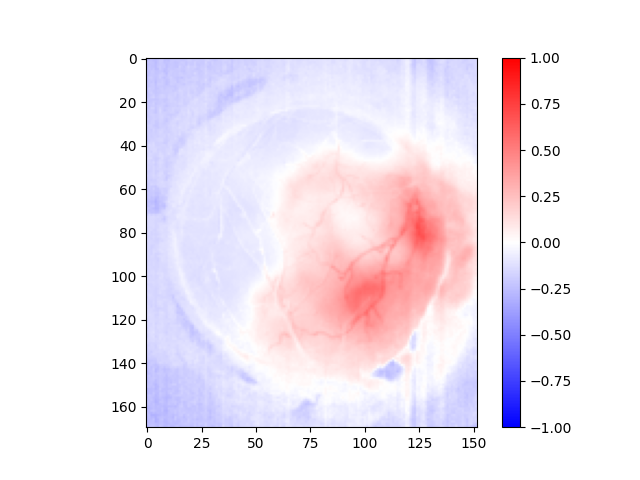
\includegraphics[scale=0.4]{m219_r25_t1/avg_strf}
	\caption{Own result}
	\label{fig:strf_m219_r25}
\end{figure}

\begin{figure}
\centering
\animategraphics[width=0.7\linewidth,controls]{30}{m219_r25_t1/video/image}{1}{31}
\caption{This figure is generated using the same data as Figure \ref{fig:strf_m219_r25} but instead the STRF of each neuron is only summed accross the spatial dimension, resulting in a video where the average STRF value is shown for each moment $t$}
\end{figure}


After applying the DSTRF algorithm described above: training the CNN network, linearizing it and multiplying the weights, an interpretable movie visualization for every pixel $p$ of the calcium imaging recording was obtained. Shown below is a selection of such movies, compressed in order to save space in the document (raw, uncompressed videos are also provided, along with the full code).

\todo{3-4 DSTRF videos with labeled trial, recording, pixel}

\begin{figure}
	\centering
	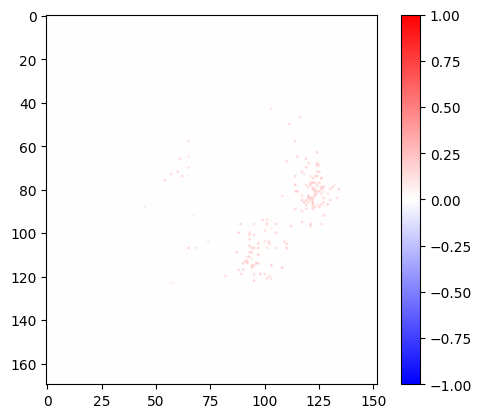
\includegraphics[scale=0.8]{50_trials}
	\caption{The figure shows the average Pearson correlation scores per pixel between the actual response to the stimulus and the response predicted by the DSTRF. It is clear that the correlation overlap with the "seed" areas of activation, as seen in the recording.}
	\label{fig:50trials}
\end{figure}

